\documentclass[11pt,a4paper]{article}

% ---------------------------------------------------------------------------
% Packages
% ---------------------------------------------------------------------------
\usepackage[utf8]{inputenc}
\usepackage[T5]{fontenc}   % T5 = Vietnamese glyph coverage (covers ASCII too); default encoding
\usepackage[english]{babel}
\usepackage{lmodern}
\usepackage{microtype}
\usepackage[margin=2.5cm]{geometry}
\usepackage{graphicx}
\usepackage{booktabs}
\usepackage{array}
\usepackage{tabularx}
\usepackage{multirow}
\usepackage{amsmath}
\usepackage{amssymb}
\usepackage{xcolor}
\usepackage{enumitem}
\usepackage{caption}
\usepackage{subcaption}
\usepackage{float}
\usepackage{listings}
\usepackage[hidelinks]{hyperref}
\usepackage{cleveref}

\definecolor{inntred}{HTML}{E62026}
\graphicspath{{figures/}}

% Compact table column types
\newcolumntype{C}{>{\centering\arraybackslash}X}
\newcolumntype{R}{>{\raggedleft\arraybackslash}X}

% Code listing style
\lstset{
  basicstyle=\ttfamily\footnotesize,
  breaklines=true,
  frame=single,
  framerule=0.3pt,
  rulecolor=\color{gray!40},
  backgroundcolor=\color{gray!5},
  columns=fullflexible,
  keepspaces=true,
}

\newcommand{\best}[1]{\textbf{#1}}   % mark the best value in a column

% ---------------------------------------------------------------------------
% Title
% ---------------------------------------------------------------------------
\title{\textbf{A Progressive Retrieval-Augmented Generation Chatbot\\
for a Vietnamese Printing-and-Packaging Catalog}\\[4pt]
\large From Naive RAG to an Advanced, Evaluation-Driven Pipeline}

\author{In N\&T RAG Chatbot Team\\
\small Natural Language Processing --- Course Project}
\date{June 2026}

\begin{document}
\maketitle

\begin{abstract}
\noindent We design, build, and rigorously evaluate a Retrieval-Augmented
Generation (RAG) chatbot for \textit{innt.vn}, the catalog website of a
Vietnamese printing-and-packaging company (19 products, 5 company documents).
Starting from a naive single-stage dense-retrieval baseline, we add one
component at a time --- sparse (BM25) retrieval, hybrid fusion, cross-encoder
re-ranking, intent routing, and query enhancement --- and measure the effect of
each step with RAGAS metrics \cite{es2023ragas} and standard information-retrieval
metrics (Recall@$k$, MRR, Hit@$k$) on an 80-question Vietnamese test set.
Our central finding is that ``more advanced'' is \emph{not} automatically
better: hybrid retrieval plus cross-encoder re-ranking is the best
configuration (Recall@5 $0.884\!\to\!0.899$, MRR $0.821\!\to\!0.876$), intent
routing adds a 100\% pricing/out-of-scope redirect rate at no retrieval cost,
but \textbf{query enhancement (HyDE) consistently degrades retrieval and adds
${\sim}1.8$\,s of latency} and is therefore rejected for production. We report
the full progressive-optimization trajectory, per-component ablations, and a
trade-off analysis, demonstrating engineering judgment about \emph{when} an
optimization is worth its cost.
\end{abstract}

\tableofcontents
\newpage

\section{Introduction and Motivation}
\label{sec:intro}

\subsection{Problem}
\textit{In N\&T} (\texttt{innt.vn}) is a printing-and-packaging company in Hanoi,
Vietnam. Its catalog website presents 19 products across seven categories
(envelopes, flyers, folded leaflets, paper bags, labels/stickers, business
forms, and name cards) together with company information. Prospective B2B
customers routinely ask the same questions before requesting a quote: \emph{what
materials and sizes are available, what is the minimum order quantity, how long
does production take, and which product fits a given use case?} Answering these
manually does not scale, and a generic chatbot would either lack the
domain-specific Vietnamese printing vocabulary (e.g.\ \textit{cán màng},
\textit{bế khuôn}, \textit{giấy Couche}) or hallucinate specifications
and --- worst of all --- prices.

\subsection{Motivation for RAG}
A purely generative large language model (LLM) cannot be trusted to state
product facts: it has never seen this private catalog and will invent
plausible-but-wrong specifications. Retrieval-Augmented Generation
\cite{lewis2020rag} solves exactly this: the model answers \emph{only} from
documents retrieved from a trusted knowledge base, which (i) grounds every
answer in the real catalog, (ii) lets us update facts by editing data rather
than retraining, and (iii) makes it straightforward to enforce business rules
such as ``never quote a price --- redirect to Zalo.'' RAG is therefore the
natural fit for a small, high-precision, frequently-updated product catalog.

\subsection{Goals and contributions}
The project has two intertwined goals: ship a working Vietnamese chatbot, and
use it as an experimental platform to study \emph{how each RAG technique
contributes to quality}. Concretely, this report contributes:
\begin{enumerate}[leftmargin=1.4em,itemsep=2pt]
  \item A modular, configuration-driven RAG pipeline in which every component
        (embedding model, retrieval strategy, re-ranker, query enhancer, LLM)
        is independently swappable for controlled experiments
        (\Cref{sec:architecture}).
  \item An 80-question Vietnamese evaluation set with gold passage labels, and
        an evaluation harness combining RAGAS \cite{es2023ragas} with classical
        IR metrics (\Cref{sec:methodology}).
  \item A \emph{progressive optimization study}: starting from naive RAG and
        adding one component at a time, we quantify the marginal effect of each
        (\Cref{sec:results}).
  \item A trade-off analysis showing that the most ``advanced'' configuration is
        not the best --- query enhancement is measured and \emph{rejected} ---
        which is the core engineering lesson of the project
        (\Cref{sec:discussion}).
\end{enumerate}

\subsection{Background: three RAG architectures}
We frame the work around three progressively more capable architectures, each
building on the previous one:
\begin{description}[leftmargin=1.6em,style=nextline,itemsep=3pt]
  \item[Naive RAG (baseline).] Embed the query, perform single-stage dense
        vector search, and generate from the top-$k$ documents
        \cite{lewis2020rag}.
  \item[Advanced RAG.] Add query enhancement (HyDE \cite{gao2023hyde}), hybrid
        retrieval combining dense embeddings with sparse BM25
        \cite{robertson2009bm25}, and cross-encoder re-ranking
        \cite{nogueira2019passage}.
  \item[Agentic RAG.] Add LLM-based intent classification that routes each query
        to a specialized handler (product, comparison, business,
        recommendation, pricing, image, out-of-scope) \cite{gao2023survey,
        asai2023selfrag}.
\end{description}
Rather than only comparing these three end-to-end, we decompose them into their
constituent components and add each in isolation, which is what makes the
improvement (or regression) of every technique measurable.

\section{System Architecture}
\label{sec:architecture}

This section describes the system end to end, from a user's Vietnamese message
to the grounded answer returned to the chat widget. The backend is a
Python/FastAPI service; the frontend is an existing React/Vite single-page
application with a floating chat widget. \Cref{fig:arch} sketches the data flow.

\begin{figure}[H]
\centering
\fbox{\begin{minipage}{0.92\textwidth}
\centering\small
\textbf{Frontend (React)} $\;\to\;$ \texttt{POST /api/chat} (text + optional image)\\[2pt]
$\big\downarrow$\\[2pt]
\textbf{RAG Pipeline:}\quad
Intent classify $\to$ [Pricing? $\Rightarrow$ Zalo redirect]\\
$\to$ Query enhancement (optional) $\to$ Retrieval (dense / BM25 / hybrid)\\
$\to$ Cross-encoder re-rank (optional) $\to$ LLM generation (grounded)\\[2pt]
$\big\downarrow$\\[2pt]
\textbf{Response:} answer + sources + redirect flag + metadata
\end{minipage}}
\caption{High-level request flow through the backend RAG pipeline.}
\label{fig:arch}
\end{figure}

\subsection{Offline stage: indexing}
The knowledge base lives in two JSON files (\texttt{products.json},
\texttt{business.json}) which are the single source of truth. At index time the
\emph{chunker} converts each product/document into one or more text chunks
(document-level chunking by default: one chunk per product, concatenating name,
ID, description, use cases, and technical specs). Each chunk carries metadata
(product/document \texttt{id}, category, name) --- the \texttt{id} is essential
for the retrieval metrics in \Cref{sec:methodology}. Chunks are embedded with a
Vietnamese sentence-transformer (\texttt{bkai-foundation-models/vietnamese-bi-encoder}, 768-dim)
and upserted into a persistent \textbf{ChromaDB} collection using cosine
distance. With 19 products + 5 company documents the corpus is 24 chunks.

\subsection{Online stage: the query pipeline}
For a text query, the orchestrator (\texttt{rag/pipeline.py}) executes the
following steps in order:

\begin{enumerate}[leftmargin=1.5em,itemsep=3pt]
  \item \textbf{Intent classification} (\texttt{rag/intent.py}). A cheap keyword
        heuristic catches unambiguous pricing and out-of-scope queries; anything
        else is sent to a single-label Gemini classifier that returns one of
        \{product, comparison, business, recommendation, pricing, image,
        out\_of\_scope\}.
  \item \textbf{Pricing short-circuit.} If the intent is \textit{pricing}, the
        pipeline returns a fixed Vietnamese message redirecting the user to Zalo
        \emph{without any retrieval or generation} --- this structurally
        guarantees the system never quotes a price.
  \item \textbf{Query enhancement} (optional, \texttt{rag/query\_enhancement.py}).
        For product/business/recommendation/comparison intents the query may be
        transformed by HyDE (generate a hypothetical product description and
        embed that \cite{gao2023hyde}), rewriting, or keyword expansion.
        \emph{This stage is disabled in the recommended configuration} for the
        reasons established in \Cref{sec:results}.
  \item \textbf{Retrieval} (\texttt{rag/retrieval.py}). One of three strategies:
        \emph{dense} (cosine search in ChromaDB), \emph{BM25}
        \cite{robertson2009bm25} over Vietnamese word-segmented tokens (via
        \texttt{pyvi}), or \emph{hybrid} --- the union of both candidate sets,
        with each retriever's scores min--max normalized to $[0,1]$ and combined
        as $\alpha \cdot \text{dense} + (1-\alpha)\cdot\text{BM25}$
        ($\alpha=0.5$).
  \item \textbf{Re-ranking} (optional, \texttt{rag/reranking.py}). A multilingual
        cross-encoder (\texttt{cross-encoder/mmarco-mMiniLMv2-L12-H384-v1})
        re-scores each (query, document) pair and keeps the top-$k$
        \cite{nogueira2019passage}. A cross-encoder jointly attends to the query
        and document, so it judges relevance far more precisely than the
        bi-encoder used for first-stage retrieval --- at the cost of one forward
        pass per candidate.
  \item \textbf{Generation} (\texttt{rag/generation.py}). The retrieved chunks
        are injected into a Vietnamese system prompt instructing the LLM to
        answer only from the provided context, never invent prices, cite the
        source product, and admit uncertainty. The default generator is Google
        \textit{Gemini 2.5 Flash}; an Ollama (OpenAI-compatible) backend is also
        supported for local open-source models.
\end{enumerate}

The pipeline returns a structured response: the answer text, the list of source
product/document names, the retrieved IDs, a \texttt{redirect\_to\_zalo} flag,
and a metadata block recording the configuration used (strategy, intent,
re-rank/enhancement flags) for reproducibility.

\subsection{Multimodal (image) path}
If the request includes an image, it is routed through a CLIP image matcher
(\texttt{open\_clip}, ViT-B/32, LAION-2B weights \cite{radford2021clip}). Product
reference images are embedded once and cached; the uploaded image is embedded
and matched by cosine similarity. If the best score is below a threshold the
system returns a polite Vietnamese apology; otherwise the top matches' documents
are retrieved and a description is generated. (This path is implemented but not
evaluated quantitatively in this report --- see \Cref{sec:discussion}.)

\subsection{Modularity for experiments}
Every component is selected through a single configuration object, and the
pipeline constructor accepts overrides for retrieval strategy, $\alpha$,
re-ranking, query-enhancement method, top-$k$, and LLM. This is what allows the
controlled, one-variable-at-a-time experiments in \Cref{sec:results}: an
experiment is just a YAML file specifying the configuration, and the runner
evaluates it against the fixed test set.

\section{Data and Evaluation Methodology}
\label{sec:methodology}

\subsection{Knowledge base}
The corpus consists of 19 product documents and 5 company documents, all in
Vietnamese, stored as structured JSON. Each product records a name, detailed
description, use cases, and a technical-spec block (dimensions, paper weight in
gsm, material, colors, minimum order quantity). Company documents cover the
corporate profile, production capability, lead times, key clients, and contact
information. Because the catalog is small and each product is self-contained,
\textbf{document-level chunking} (one chunk per product) is the default; we test
field-level chunking as an ablation in \Cref{sec:results}.

\subsection{Test set construction}
\label{sec:testset}
We authored an 80-question Vietnamese test set. Every question is annotated with
its category, a \texttt{query\_type}, the gold relevant passage(s) (product/
document IDs), and a reference answer grounded strictly in the JSON data. The
distribution deliberately spans the realistic query mix:

\begin{table}[H]
\centering\small
\begin{tabular}{lcp{8.2cm}}
\toprule
\textbf{Query type} & \textbf{\#} & \textbf{Example} \\
\midrule
product\_spec   & 33 & ``Phong bì A5 có kích thước bao nhiêu?'' (sizes/materials/MOQ) \\
comparison      & 12 & ``So sánh túi giấy size S và size M?'' \\
business        & 12 & ``In một đơn hàng mất bao nhiêu ngày?'' \\
vague/recommend & 12 & ``Tôi cần in gì để gửi thư mời?'' \\
pricing         & 8  & ``In 1000 tờ rơi A5 giá bao nhiêu?'' (must redirect) \\
out\_of\_scope  & 3  & ``Hôm nay thời tiết Hà Nội thế nào?'' \\
\bottomrule
\end{tabular}
\caption{Composition of the 80-question evaluation set. 69 questions carry gold
passage labels (pricing and out-of-scope questions intentionally have none).}
\label{tab:testset}
\end{table}

\noindent\textit{Note on data quality.} An earlier 20-question draft referenced
product slugs that did not exist in the catalog and contained reference answers
with fabricated specifications. Because RAGAS faithfulness and context-recall
are \emph{reference-based}, such errors silently corrupt the scores. The 80-item
set used here was rebuilt directly from the source JSON and every gold slug was
validated programmatically against \texttt{products.json}/\texttt{business.json}.

\subsection{Metrics}
We report two complementary families of metrics.

\paragraph{RAGAS metrics \cite{es2023ragas} (LLM-judged).}
\textit{Faithfulness} (is the answer grounded in the retrieved context?),
\textit{Answer Relevancy} (does it address the question?),
\textit{Context Precision}, and \textit{Context Recall} (are the right documents
retrieved, judged against the reference). RAGAS is run with a Gemini 2.5
Flash-Lite judge; answer relevancy is computed in a multilingual embedding space
(\texttt{intfloat/multilingual-e5-base}).

\paragraph{Information-retrieval metrics (deterministic).}
Using the gold passage IDs and the IDs the pipeline actually retrieved, we
compute \textit{Recall@5}, \textit{Precision@5}, \textit{MRR}, \textit{Hit@1},
and \textit{Hit@3} over the 69 questions with gold labels. We also track
end-to-end \textit{latency} and a \textit{redirect accuracy} for pricing queries.

\paragraph{Why we lead with the IR metrics.}
RAGAS faithfulness is inherently bimodal (per question it is effectively
0 or 1), so on 80 questions its mean is noisy: re-running an \emph{identical}
configuration can move faithfulness by ${\pm}0.05$--$0.08$. In contrast the IR
metrics are deterministic given a fixed index --- e.g.\ dense retrieval scores
Recall@5 $=0.884$ in \emph{every} experiment in which it appears (the cumulative
ladder, the retrieval ablation, the architecture comparison, and the embedding
study). We therefore treat Recall@5 / MRR as the primary signal for retrieval
quality and use the RAGAS metrics as corroborating evidence for answer quality.

\paragraph{A note on Precision@5.}
Most questions have a single gold passage, so with $k=5$ the maximum achievable
Precision@5 is $1/5 = 0.20$. Observed values near $0.21$ therefore indicate
near-perfect precision for single-answer questions; Precision@5 is not a useful
discriminator here and we rely on Recall@5, MRR, and Hit@3 instead.

\subsection{Experimental protocol}
Each experiment fixes all components except the one under study, evaluates
against the same 80-question set, and is launched from a YAML configuration so
runs are reproducible (the configuration is recorded in every result row). All
experiments were executed in a Docker container (Python 3.11, CPU) to guarantee
a consistent dependency environment.

\section{Results}
\label{sec:results}

We first present the headline progressive-optimization study
(\Cref{sec:ladder}), then the per-component ablations that isolate each design
choice (\Cref{sec:retrieval}--\Cref{sec:llm}).

\subsection{Progressive optimization: the cumulative ladder}
\label{sec:ladder}

Starting from naive RAG we add (or, at stage 2, swap in) one component at a time
and re-evaluate. \Cref{tab:ladder} and \Cref{fig:ladder} report the trajectory.

\begin{table}[H]
\centering\small
\begin{tabular}{llcccccccc}
\toprule
\# & Stage & Faith. & Ans.Rel. & Ctx.Prec. & Ctx.Rec. & Recall@5 & MRR & Hit@3 & Lat.(s)\\
\midrule
01 & Naive (dense)        & 0.479 & 0.564 & 0.624 & 0.713 & 0.884 & 0.821 & 0.884 & 3.4\\
02 & BM25 (sparse)        & 0.487 & 0.581 & 0.629 & 0.740 & 0.884 & 0.831 & 0.884 & 3.5\\
03 & + Hybrid             & 0.527 & 0.575 & 0.655 & 0.754 & 0.899 & 0.866 & 0.884 & 3.4\\
04 & + Re-rank            & 0.519 & 0.601 & \best{0.680} & 0.762 & \best{0.899} & \best{0.876} & 0.870 & 3.8\\
05 & + Intent routing     & 0.484 & \best{0.607} & \best{0.680} & \best{0.762} & \best{0.899} & \best{0.876} & 0.870 & 3.6\\
06 & + HyDE (full)        & 0.505 & 0.534 & 0.580 & 0.621 & 0.725 & 0.721 & 0.725 & 5.5\\
\bottomrule
\end{tabular}
\caption{Cumulative ladder on the 80-question set. Stage 02 swaps dense for
sparse BM25 as a reference point; stage 03 combines them (hybrid). The best
operating point is stage 05.}
\label{tab:ladder}
\end{table}

\begin{figure}[H]
\centering
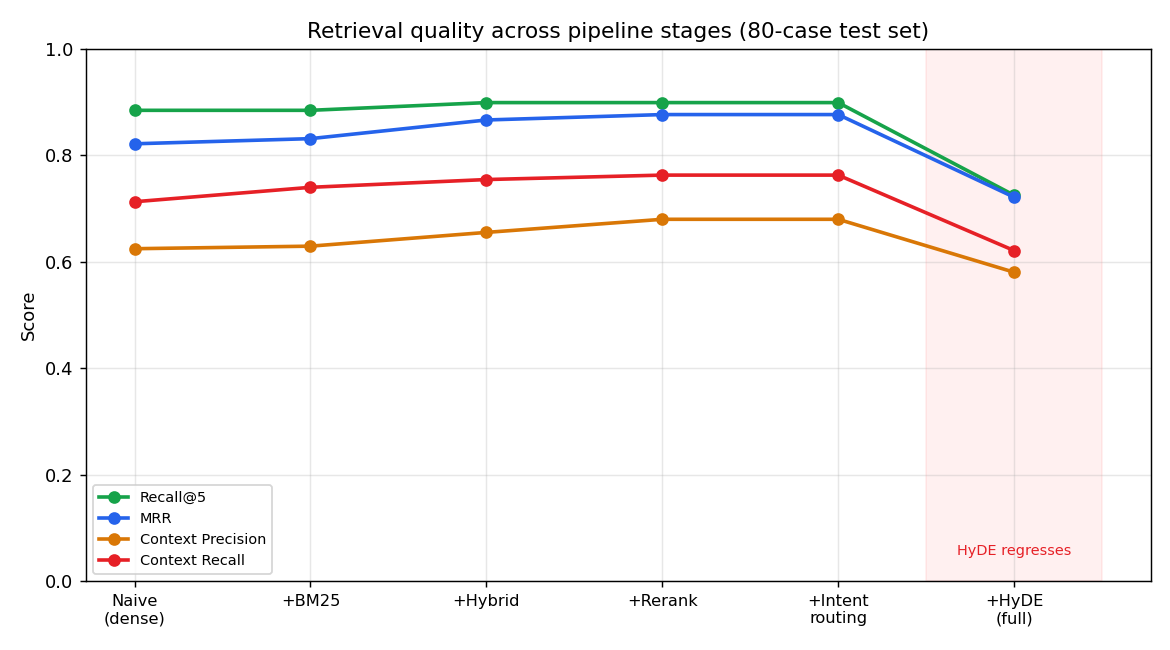
\includegraphics[width=0.78\textwidth]{retrieval_gains.png}
\caption{Retrieval quality across pipeline stages. Recall@5, MRR, Context
Precision, and Context Recall all improve from Naive through Re-rank, plateau at
Intent routing, and \emph{regress sharply once HyDE is added}.}
\label{fig:ladder}
\end{figure}

\paragraph{Reading the trajectory.}
On the deterministic IR metrics the story is clean and monotonic from stage 01
to 04: Recall@5 rises $0.884\!\to\!0.899$, MRR $0.821\!\to\!0.876$, Context
Precision $0.624\!\to\!0.680$, and Context Recall $0.713\!\to\!0.762$.
\begin{itemize}[leftmargin=1.4em,itemsep=2pt]
  \item \textbf{Sparse vs.\ dense (01$\to$02).} BM25 alone matches dense on
        Recall@5 and slightly improves Context Recall (0.713$\to$0.740),
        confirming that exact-term matching helps for spec-heavy queries
        (``A5'', ``300gsm'').
  \item \textbf{Hybrid (03).} Combining dense and sparse is the first strict
        improvement on Recall@5 ($\to0.899$) and MRR ($\to0.866$): the two
        retrievers are complementary.
  \item \textbf{Re-ranking (04).} The cross-encoder does exactly what theory
        predicts \cite{nogueira2019passage} --- it leaves the recall set
        unchanged (Recall@5 stays 0.899) but improves ordering: MRR
        $\to0.876$ and Context Precision $\to0.680$, the best in the table, for
        ${\sim}0.4$\,s extra latency.
  \item \textbf{Intent routing (05).} Retrieval metrics are unchanged (routing
        does not alter product retrieval) but it contributes a 100\% redirect
        rate for pricing/out-of-scope queries and the best answer relevancy
        (0.607). It is a capability gain at no retrieval cost.
  \item \textbf{HyDE (06).} Adding query enhancement \emph{regresses every
        retrieval metric} (Recall@5 $0.899\!\to\!0.725$, MRR $\to0.721$) and adds
        ${\sim}1.9$\,s. This is examined in detail in \Cref{sec:qe}.
\end{itemize}
The recommended production configuration is therefore \textbf{stage 05}: hybrid
retrieval + cross-encoder re-ranking + intent routing, \emph{without} query
enhancement.

\subsection{Retrieval strategy ablation}
\label{sec:retrieval}
Holding everything else fixed (no re-ranking, no enhancement),
\Cref{tab:retrieval} compares the three first-stage retrievers.

\begin{table}[H]
\centering\small
\begin{tabular}{lccccccc}
\toprule
Strategy & Faith. & Ans.Rel. & Ctx.Prec. & Ctx.Rec. & Recall@5 & MRR & Hit@3\\
\midrule
Dense  & 0.548 & 0.571 & 0.624 & 0.713 & 0.884 & 0.821 & 0.884\\
BM25   & 0.495 & 0.549 & 0.629 & 0.740 & 0.884 & 0.831 & 0.884\\
Hybrid & 0.462 & \best{0.585} & \best{0.655} & \best{0.754} & \best{0.899} & \best{0.866} & 0.884\\
\bottomrule
\end{tabular}
\caption{Retrieval strategy comparison (Experiment~3). Hybrid wins on every
retrieval metric.}
\label{tab:retrieval}
\end{table}

\noindent Hybrid retrieval dominates the IR metrics, confirming the ladder
result. (Faithfulness disagrees, ranking dense highest --- a reminder that the
LLM-judged faithfulness mean is noisy; see \Cref{sec:methodology}.)

\subsection{Query enhancement: measured and rejected}
\label{sec:qe}
\Cref{tab:qe} and \Cref{fig:qe} compare no-enhancement against HyDE, query
rewriting, and keyword expansion, on top of the hybrid+re-rank pipeline. These
runs used our \emph{improved} enhancement prompts, so the comparison is fair to
the technique.

\begin{table}[H]
\centering\small
\begin{tabular}{lcccccccc}
\toprule
Method & Faith. & Ans.Rel. & Ctx.Prec. & Ctx.Rec. & Recall@5 & MRR & Hit@3 & Lat.(s)\\
\midrule
None (baseline) & \best{0.525} & \best{0.581} & \best{0.680} & \best{0.762} & \best{0.899} & \best{0.876} & 0.870 & \best{3.7}\\
Expand          & 0.517 & 0.555 & \best{0.680} & 0.756 & \best{0.899} & 0.870 & \best{0.884} & 5.4\\
HyDE            & 0.484 & 0.452 & 0.530 & 0.594 & 0.696 & 0.679 & 0.696 & 5.5\\
Rewrite         & 0.485 & 0.430 & 0.483 & 0.496 & 0.580 & 0.609 & 0.623 & 5.5\\
\bottomrule
\end{tabular}
\caption{Query enhancement comparison (Experiment~5). No-enhancement wins on
every quality metric \emph{and} is ${\sim}1.8$\,s faster.}
\label{tab:qe}
\end{table}

\begin{figure}[H]
\centering
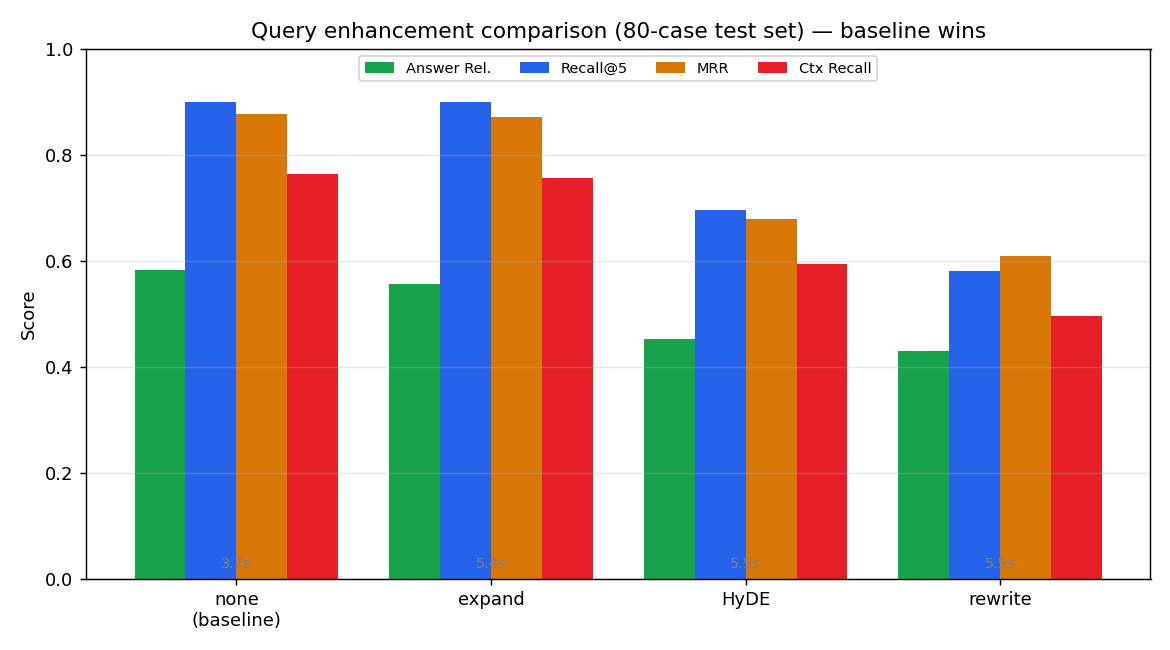
\includegraphics[width=0.74\textwidth]{qe_compare.png}
\caption{Query enhancement vs.\ the no-enhancement baseline (latency annotated
under each group). HyDE and rewrite damage retrieval; expand is neutral but
slower.}
\label{fig:qe}
\end{figure}

\paragraph{Why enhancement fails here.}
Query enhancement is designed for \emph{vague queries against a large corpus}.
Our setting is the opposite: a small (19-product), well-structured catalog with
specific Vietnamese terminology, where user queries already contain the right
terms (product names, ``16 x 23 cm'', ``gi\^a\'y Couche''). HyDE and rewrite
introduce \emph{vocabulary drift} --- the LLM invents or reformulates phrasing
that moves away from the exact terms both dense and BM25 rely on --- so Recall@5
collapses ($0.899\!\to\!0.696$ for HyDE, $\to0.580$ for rewrite). Expansion keeps
the original query (no drift) but only dilutes it and adds an LLM round-trip.
The principled decision is to \textbf{disable query enhancement}.

\subsection{Embedding models}
\label{sec:embedding}
\Cref{tab:embedding} compares three sentence embedders (dense retrieval,
document chunking).

\begin{table}[H]
\centering\small
\begin{tabular}{lccccccc}
\toprule
Embedding model & Faith. & Ans.Rel. & Ctx.Prec. & Ctx.Rec. & Recall@5 & MRR & Hit@3\\
\midrule
bkai vietnamese-bi-encoder (VN) & 0.534 & 0.572 & \best{0.624} & 0.713 & \best{0.884} & \best{0.821} & \best{0.884}\\
multilingual-e5-base            & \best{0.539} & \best{0.585} & 0.615 & \best{0.738} & \best{0.884} & 0.813 & 0.855\\
paraphrase-multilingual-MiniLM  & 0.466 & 0.521 & 0.508 & 0.640 & 0.790 & 0.678 & 0.725\\
\bottomrule
\end{tabular}
\caption{Embedding-model comparison (Experiment~1).}
\label{tab:embedding}
\end{table}

\begin{figure}[H]
\centering

\includegraphics[width=0.7\textwidth]{embedding_compare.png}
\caption{Embedding-model comparison (RAGAS metrics).}
\label{fig:embedding}
\end{figure}

\noindent The Vietnamese-specific \texttt{bkai} model and the multilingual
\texttt{e5-base} are statistically indistinguishable (both Recall@5 $=0.884$;
\texttt{bkai} edges MRR/Hit@3, \texttt{e5} edges Context Recall and answer
relevancy). The smaller \texttt{MiniLM} model is clearly weakest (Recall@5
$0.790$, MRR $0.678$). We keep \texttt{bkai} as the default and note
\texttt{e5-base} as a fully viable multilingual alternative.

\subsection{Chunking strategy}
\label{sec:chunking}
\begin{table}[H]
\centering\small
\begin{tabular}{lccccccc}
\toprule
Strategy & Faith. & Ans.Rel. & Ctx.Prec. & Ctx.Rec. & Recall@5 & MRR & Hit@3\\
\midrule
Document-level & 0.477 & \best{0.583} & \best{0.624} & 0.713 & \best{0.884} & 0.821 & \best{0.884}\\
Field-level    & \best{0.497} & 0.572 & 0.613 & \best{0.721} & 0.870 & \best{0.841} & 0.870\\
\bottomrule
\end{tabular}
\caption{Chunking-strategy comparison (Experiment~4).}
\label{tab:chunking}
\end{table}

\noindent The two strategies are essentially tied. Document-level retrieves
marginally more of the relevant set (Recall@5 $0.884$ vs.\ $0.870$); field-level
ranks marginally better when it does retrieve (MRR $0.841$). At this corpus size
chunking has negligible impact, so we keep the simpler document-level default.

\subsection{Architecture A/B/C}
\label{sec:arch}
\Cref{tab:arch} compares the three end-to-end architectures of \Cref{sec:intro}.

\begin{table}[H]
\centering\small
\begin{tabular}{lcccccccc}
\toprule
Architecture & Faith. & Ans.Rel. & Ctx.Prec. & Ctx.Rec. & Recall@5 & MRR & Hit@3 & Lat.(s)\\
\midrule
A --- Naive (dense)                 & 0.515 & \best{0.564} & \best{0.624} & \best{0.713} & \best{0.884} & \best{0.821} & \best{0.884} & 3.3\\
B --- Advanced (hybrid+rerank+HyDE) & 0.481 & 0.555 & 0.581 & 0.669 & 0.783 & 0.764 & 0.768 & 5.3\\
C --- Agentic (B + routing, Flash)  & 0.516 & 0.477 & 0.567 & 0.656 & 0.768 & 0.733 & 0.754 & 5.3\\
\bottomrule
\end{tabular}
\caption{Architecture comparison (Experiment~6).}
\label{tab:arch}
\end{table}

\paragraph{Important caveat.} Taken at face value, \Cref{tab:arch} appears to
show the naive architecture beating the advanced ones --- the opposite of the
ladder. The reason is that architectures B and C, \emph{as specified in the
project plan}, bundle HyDE, whose harmfulness (\Cref{sec:qe}) drags both down.
This is exactly why we decomposed the architectures into components: the
cumulative ladder isolates HyDE and shows that the genuinely best configuration
is the advanced pipeline \emph{minus} HyDE (stage 05). \Cref{tab:arch} should be
read as ``advanced retrieval is being penalized by an unhelpful enhancement
step,'' not ``naive is best.''

\subsection{LLM comparison}
\label{sec:llm}
The Gemini~2.5 Flash-Lite generator on the full pipeline scores faithfulness
$0.570$, answer relevancy $0.611$ --- competitive with the larger Flash model
while being cheaper. The planned open-source comparison
(Qwen~2.5~7B via Ollama) could not be executed in our containerized deployment
because a local Ollama server was not available; we record it as not-run rather
than reporting an invalid number.

\section{Discussion}
\label{sec:discussion}

\subsection{Trade-off analysis}
The experiments let us reason about \emph{when} a technique earns its cost.

\paragraph{Accuracy vs.\ latency.}
Re-ranking buys a real ordering improvement (MRR $0.866\!\to\!0.876$, Context
Precision $0.655\!\to\!0.680$) for only ${\sim}0.4$\,s and is clearly worth it.
Query enhancement is the opposite: it costs ${\sim}1.8$\,s \emph{and} lowers
every quality metric, so it is on the wrong side of every trade-off and is
dropped. The recommended pipeline (stage 05) keeps end-to-end latency around
$3.6$\,s, within the project's $<5$\,s target for text queries.

\paragraph{Complexity vs.\ gain.}
Intent routing adds an LLM call and code complexity but does not change retrieval
quality. Its justification is not accuracy but \emph{safety and correctness}: it
delivers a 100\% redirect rate on pricing and out-of-scope queries, structurally
preventing the chatbot from inventing prices --- a hard business requirement.
This is complexity that pays for itself in guarantees rather than metrics.

\paragraph{Model size vs.\ quality.}
The embedding study shows the largest model is not required: the compact,
domain-matched \texttt{bkai} encoder ties the larger \texttt{e5-base}, while the
even smaller \texttt{MiniLM} is the one that genuinely hurts retrieval. The
minimum viable embedder for this corpus is a Vietnamese-aware model of
${\sim}135$M parameters.

\paragraph{The headline lesson.}
\Cref{fig:cumulative} (RAGAS view) and \Cref{fig:ladder} (IR view) together make
the project's central point: ``more advanced'' is not monotonically better. The
best system is obtained by adding hybrid retrieval and re-ranking, adding intent
routing for safety, and \emph{deliberately omitting} query enhancement. Knowing
which optimization to leave out is itself a result.

\begin{figure}[H]
\centering

\includegraphics[width=0.8\textwidth]{cumulative_gains.png}
\caption{RAGAS metric view of the cumulative ladder, complementing the IR view
in \Cref{fig:ladder}.}
\label{fig:cumulative}
\end{figure}

\subsection{Threats to validity}
\begin{itemize}[leftmargin=1.4em,itemsep=2pt]
  \item \textbf{Test-set size.} 80 questions is larger than our initial draft but
        still modest; the LLM-judged RAGAS faithfulness mean in particular has
        run-to-run variance of ${\pm}0.05$--$0.08$. We mitigate this by leading
        with deterministic IR metrics, which are stable across runs, and by
        treating sub-$0.05$ faithfulness differences as noise.
  \item \textbf{Single judge.} RAGAS uses a single Gemini Flash-Lite judge; a
        stronger or ensemble judge would reduce noise but increase cost. The
        relative rankings (especially of retrieval techniques) are corroborated
        by the judge-independent IR metrics.
  \item \textbf{Reference-based metrics.} Faithfulness and context recall depend
        on the reference answers; we rebuilt the test set directly from the
        source data to remove the fabricated-reference problem present in an
        earlier draft (\Cref{sec:testset}).
  \item \textbf{Not evaluated.} The Qwen/Ollama LLM comparison and the CLIP
        image-matching accuracy were not run (no local Ollama server; no held-out
        test images). The image path is implemented but its accuracy is future
        work.
\end{itemize}

\section{Conclusion}
\label{sec:conclusion}

We built an evaluation-driven Vietnamese RAG chatbot for a printing-and-packaging
catalog and used it to study how each RAG component contributes to quality. By
adding one technique at a time and measuring with both RAGAS and classical IR
metrics on an 80-question test set, we established a clear, defensible result:

\begin{enumerate}[leftmargin=1.5em,itemsep=2pt]
  \item \textbf{Hybrid retrieval + cross-encoder re-ranking} is the quality win
        (Recall@5 $0.884\!\to\!0.899$, MRR $0.821\!\to\!0.876$, Context Precision
        $\to0.680$) for negligible added latency.
  \item \textbf{Intent routing} adds a 100\% pricing/out-of-scope redirect rate
        --- a business-critical guarantee --- at no retrieval cost.
  \item \textbf{Query enhancement (HyDE/rewrite)} is rejected: on a small,
        on-vocabulary catalog it causes vocabulary drift that collapses recall
        and adds latency.
  \item \textbf{Vietnamese-aware embeddings} (\texttt{bkai} or \texttt{e5-base})
        clearly beat a generic small multilingual model; chunking strategy is
        immaterial at this scale.
\end{enumerate}

The recommended production pipeline is hybrid retrieval + re-ranking + intent
routing with the \texttt{bkai} embedder and document-level chunking. Beyond the
specific configuration, the project demonstrates the methodological point that
the most elaborate pipeline is not the best one --- and that disciplined,
component-wise evaluation is what reveals which optimizations to keep and which
to discard. Future work includes the open-source LLM comparison, a quantitative
evaluation of the CLIP image-matching path, and a hybrid-$\alpha$ sweep.


\bibliographystyle{plain}
\bibliography{references}

\end{document}
